\documentclass[10pt]{article}
\usepackage{amsmath}
\usepackage{geometry}
\usepackage{fancybox}
\usepackage{amsfonts}
\usepackage{amsbsy}
\usepackage{tikz}
\usepackage{listings}
\geometry{
a4paper,
total={170mm,257mm},
left=20mm,
top=10mm,
bottom=15mm
}
\usepackage{color}
\definecolor{codegreen}{rgb}{0,0.6,0}
\definecolor{codegray}{rgb}{0.5,0.5,0.5}
\definecolor{codepurple}{rgb}{0.58,0,0.82}
\definecolor{backcolour}{rgb}{0.95,0.95,0.92}

\linespread{1.3}

\title{CSC263H1 Assignment 6}
\author{Jiatao Xiang, Xu Wang, Huakun Shen}
\date{March 28th, 2019}

\begin{document}

\lstdefinestyle{mystyle}{
    backgroundcolor=\color{backcolour},   
    commentstyle=\color{codegreen},
    keywordstyle=\color{magenta},
    numberstyle=\tiny\color{codegray},
    stringstyle=\color{codepurple},
    basicstyle=\footnotesize,
    breakatwhitespace=false,         
    breaklines=true,                 
    captionpos=b,                    
    keepspaces=true,                 
    numbers=left,                    
    numbersep=5pt,                  
    showspaces=false,                
    showstringspaces=false,
    showtabs=false,                  
    tabsize=4
}
\lstset{style=mystyle}
\maketitle
\section*{Question 1}
\begin{itemize}
\item[a.]
\end{itemize}
\ovalbox{
\begin{tikzpicture}[level/.style={sibling distance=60mm/#1}]
\node [circle,draw, label=right:$1/12$] (z){$1$}
  child {node [circle,draw, label=right:$2/3$] (lz) {$6$}}
  child {node [circle,draw, label=right:$4/11$] (rz) {$4$}
    child {node [circle,draw, label=right:$5/8$] (rlz) {$5$}
    	child {node [circle, draw, label=right:$2/3$] (rllz) {$2$}}
		child[fill=none]{edge from parent[draw=none]}     
    }
  child {node [circle,draw, label=right:$9/10$] (rrz) {$7$}
	}
};
\end{tikzpicture}
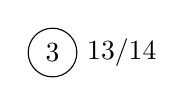
\begin{tikzpicture}[level/.style={sibling distance=60mm/#1}]
\node [circle,draw, label=right:$13/14$] (z){$3$};
\end{tikzpicture}
}
\begin{itemize}
\item[b.] Forward edge: 7, Back edge: 0, Cross edge: 5.
\item[c.] Use white-path theorem and parenthesis theorem. 
\item[d.]
\item[e.]
\end{itemize}

\section*{Question 2}


\section*{Question 3}


\end{document}
